\chapter{Optimization Theory}
\label{chapter:OptimizationTheory}

As promised in this thesis' introduction in chapter \ref{chapter:Intro}, the
Reinforcement Learning Problem is primarliy a problem in optimization. The
entire framing of finding increasingly best ways to navigate the probleem
described is based on the theory of mathematical optimization. This chapter aims
to provide a suitable framing for the remaining chapters, spinning a narrative
thread that connects all the problems to come. We focus less on specific results
and more on their meaning and geometric interpretation.

\section{Optimization as a geometry problem}

In the broadest possible terms, optimizations problems are seach problems. Such
search problems are often embedded in a geometrical context.

\begin{wrapfigure}{I}{0.5\textwidth}
   \centering
   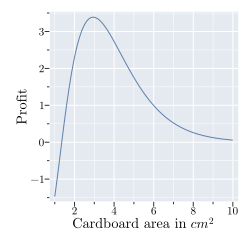
\includegraphics[width=0.5\textwidth]{img/1d-profits.tikz} 
   \caption{Profits function for the box-making company.}
   \label{fig:1d-profits}
\end{wrapfigure}

For an introductory problem, picture a company designing boxes. They have
conducted a study and isolated a relationship that describes their profits as a
function of the volume of their best-selling box. That relationship is plotted
in figure \ref{fig:1d-profits}. This company wants to maximize profit by
modifying the variable they can control: the volume of the box.

Picture for a moment that the graph shown in figure \ref{fig:1d-profits} is
unknown to the company (optimizing agent or agent henceforth), as graphical
representations are often not possible in other problems. By plotting the profit
function that is represented by some $f: \R \to \R$ finding the point that
maximizes profit is very straightforward. But since the optimizing agent does
not have this luxury, it must come up with a different strategy. The agent
recalled that derivatives have a very useful geometric interpretation, they give
the slope of a function at a point. The agent can start by guessing a value for
the volume, and then find the point where it equals zero. The logic behind the
search for a zero is simple: if a function is continuous and ``goes up'' on a
certain subset of numbers, and then ``goes down'' for the numbers right next, a
peak is necessarily in between those two regions. That peak corresponds to the
point where the derivative equals zero.

\begin{wrapfigure}{I}{0.5\textwidth}
   \centering
   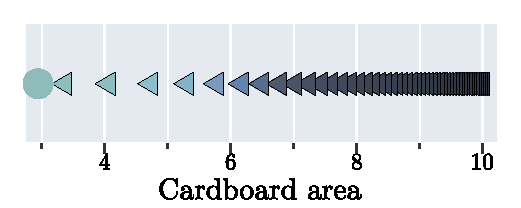
\includegraphics[width=0.5\textwidth]{img/gd-points.pdf} 
   \caption{Points the learning agent tried.}
   \label{fig:gd-points}
\end{wrapfigure}

With this in mind, the agent devises an ``educated guess'' algorithm to find the
point where the derivative equals zero, which is exactly where the peak of the
profits function is, as exemplified in figure \ref{fig:1d-profits}. The guessing
starts at the point where volume equals 10. The agent evaluates the derivative
there, and finds that it is less than zero. In other words, the profits would
diminish if he were to try a volume less than 10. So, the agent decreases the
volume to another point that is smaller by $\alpha$. The agent continues this
process changing the value $\alpha$ as it goes. Figure \ref{fig:gd-points} shows
the points this agent tried while trying to achieve a maximum. The color of the
point gets lighter as it approaches the maximum. The markers show the direction
in where the next exploration point will be, the stopping point is marked by the
circle.

Most computational methods for optimization rely on the same basic ideas as our
``educated guess'' algorithm. Since exact solutions are too computationally
expensive to calculate, or even impossible on some instances, optimization
algorithms take starting points in the seach space where an optimal point would
be found, and explore that space iteratively by means of some mechanism where
each new iteration is closer to an optimal point than the previous one. In the
case of the algorithm described so far the mechanism to approach optimality is
based on the observation that peaks correspond to zeroes of the derivative of
the function being optimized (objective function).

The algorithm we have been calling ``educated guess'' is in fact known as the
gradient descent. A ``gradient'' is the generalization of the concept of a
derivative for functions of the form $f: \R^{n} \to \R$. Let us define gradient
descent by defining an operator $D$ that acts on points in $\R^{n}$. We choose
to present the algorithm in terms of operators as it makes more palletable some
crucial ideas in chapter \ref{chapter:ApproximateLinearP}.

\begin{dfn}{Gradient Descent Operator}{}
    We define the \emph{gradient descent} operator, denoted by $D: \R^{n} \to
    \R^{n}$ for a given function $f: \R^{n} \to \R$ as
    \[
        D \vec{x} = \vec{x} - \alpha \nabla f(\vec{x}).
    \]
\end{dfn}

By using the Gradient Descent Operator, we can define a succession
$\{\vec{a}_n\}$ of points in $\R^{n}$. The succession is defined as
$\vec{a}_{n+1} = \vec{a}_n - \alpha_n \nabla f(\vec{a}_n)$. By thinking of the
process in terms of operators, finding optimal points (as they may not be
unique) is simply finding points that satisfy
\[
    D \a_* = a_*.
\]
In other words, \emph{fixed points} of the operator $D$. It can be proved that
such a fixed point exists whenever $f$ satisfies a certain set of conditions,
but reviewing it now would be besides the point. 

Some defining characteristics of the problem gradient descent solves are:
\begin{itemize}
    \item The objective function must be differentiable and unchanging
        throughout the process.
    \item The space being searched for optimal solutions is free of any
        restrictions.
    \item The exploration process has no effect on the optimal solution to be
        found. In contrast, some problems have different, branching possibilities.
        In the case described here, if an optimal solution exists it is fixed and
        cannot be altered.
\end{itemize}

[Aqui algo de simplex quizá, para introducir el concepto de restricciones. Creo
que con eso basta]


% \begin{remark}{Greedy}
%     Hola   
% \end{remark}

% \begin{remark}{Big `O' notation}
%     Hola
% \end{remark}